\documentclass[oneside]{book}

\usepackage{amsmath, amsthm, amssymb, amsfonts}
\usepackage{thmtools}
\usepackage{graphicx}
\usepackage{setspace}
\usepackage{geometry}
\usepackage{float}
\usepackage{hyperref}
\usepackage[utf8]{inputenc}
\usepackage[english]{babel}
\usepackage{framed}
\usepackage[dvipsnames]{xcolor}
\usepackage{environ}
\usepackage{tcolorbox}
\tcbuselibrary{theorems,skins,breakable}
\usepackage[UTF8]{ctex}

\usepackage{quiver} % to draw commutative diagrams

\setstretch{1.2}
\geometry{
    textheight=9in,
    textwidth=5.5in,
    top=1in,
    headheight=12pt,
    headsep=25pt,
    footskip=30pt
}

% Variables
\def\notetitle{Combinatorial Mathematics Notes}
\def\noteauthor{
    by Flaricy\\
    Peking University}
\def\notedate{Spring Semester, 2024}

% The theorem system and user-defined commands
% Theorem System
% The following boxes are provided:
%   Definition:     \defn 
%   Theorem:        \thm 
%   Lemma:          \lem
%   Corollary:      \cor
%   Proposition:    \prop   
%   Claim:          \clm
%   Fact:           \fact
%   Proof:          \pf
%   Example:        \ex
%   Remark:         \rmk (sentence), \rmkb (block)
% Suffix
%   r:              Allow Theorem/Definition to be referenced, e.g. thmr
%   p:              Add a short proof block for Lemma, Corollary, Proposition or Claim, e.g. lemp
%                   For theorems, use \pf for proof blocks

% Definition
\newtcbtheorem[number within=section]{mydefinition}{Definition}
{
    enhanced,
    frame hidden,
    titlerule=0mm,
    toptitle=1mm,
    bottomtitle=1mm,
    fonttitle=\bfseries\large,
    coltitle=black,
    colbacktitle=green!20!white,
    colback=green!10!white,
}{defn}

\NewDocumentCommand{\defn}{m+m}{
    \begin{mydefinition}{#1}{}
        #2
    \end{mydefinition}
}

\NewDocumentCommand{\defnr}{mm+m}{
    \begin{mydefinition}{#1}{#2}
        #3
    \end{mydefinition}
}

% Theorem
\newtcbtheorem[use counter from=mydefinition]{mytheorem}{Theorem}
{
    enhanced,
    frame hidden,
    titlerule=0mm,
    toptitle=1mm,
    bottomtitle=1mm,
    fonttitle=\bfseries\large,
    coltitle=black,
    colbacktitle=cyan!20!white,
    colback=cyan!10!white,
}{thm}

\NewDocumentCommand{\thm}{m+m}{
    \begin{mytheorem}{#1}{}
        #2
    \end{mytheorem}
}

\NewDocumentCommand{\thmr}{mm+m}{
    \begin{mytheorem}{#1}{#2}
        #3
    \end{mytheorem}
}

% Lemma
\newtcbtheorem[use counter from=mydefinition]{mylemma}{Lemma}
{
    enhanced,
    frame hidden,
    titlerule=0mm,
    toptitle=1mm,
    bottomtitle=1mm,
    fonttitle=\bfseries\large,
    coltitle=black,
    colbacktitle=violet!20!white,
    colback=violet!10!white,
}{lem}

\NewDocumentCommand{\lem}{m+m}{
    \begin{mylemma}{#1}{}
        #2
    \end{mylemma}
}

\newenvironment{lempf}{
	{\noindent{\it \textbf{Proof for Lemma}}}
	\tcolorbox[blanker,breakable,left=5mm,parbox=false,
    before upper={\parindent15pt},
    after skip=10pt,
	borderline west={1mm}{0pt}{violet!20!white}]
}{
    \textcolor{violet!20!white}{\hbox{}\nobreak\hfill$\blacksquare$} 
    \endtcolorbox
}

\NewDocumentCommand{\lemp}{m+m+m}{
    \begin{mylemma}{#1}{}
        #2
    \end{mylemma}

    \begin{lempf}
        #3
    \end{lempf}
}

% Corollary
\newtcbtheorem[use counter from=mydefinition]{mycorollary}{Corollary}
{
    enhanced,
    frame hidden,
    titlerule=0mm,
    toptitle=1mm,
    bottomtitle=1mm,
    fonttitle=\bfseries\large,
    coltitle=black,
    colbacktitle=orange!20!white,
    colback=orange!10!white,
}{cor}

\NewDocumentCommand{\cor}{+m}{
    \begin{mycorollary}{}{}
        #1
    \end{mycorollary}
}

\newenvironment{corpf}{
	{\noindent{\it \textbf{Proof for Corollary.}}}
	\tcolorbox[blanker,breakable,left=5mm,parbox=false,
    before upper={\parindent15pt},
    after skip=10pt,
	borderline west={1mm}{0pt}{orange!20!white}]
}{
    \textcolor{orange!20!white}{\hbox{}\nobreak\hfill$\blacksquare$} 
    \endtcolorbox
}

\NewDocumentCommand{\corp}{m+m+m}{
    \begin{mycorollary}{}{}
        #1
    \end{mycorollary}

    \begin{corpf}
        #2
    \end{corpf}
}

% Proposition
\newtcbtheorem[use counter from=mydefinition]{myproposition}{Proposition}
{
    enhanced,
    frame hidden,
    titlerule=0mm,
    toptitle=1mm,
    bottomtitle=1mm,
    fonttitle=\bfseries\large,
    coltitle=black,
    colbacktitle=yellow!30!white,
    colback=yellow!20!white,
}{prop}

\NewDocumentCommand{\prop}{+m}{
    \begin{myproposition}{}{}
        #1
    \end{myproposition}
}

\newenvironment{proppf}{
	{\noindent{\it \textbf{Proof for Proposition.}}}
	\tcolorbox[blanker,breakable,left=5mm,parbox=false,
    before upper={\parindent15pt},
    after skip=10pt,
	borderline west={1mm}{0pt}{yellow!30!white}]
}{
    \textcolor{yellow!30!white}{\hbox{}\nobreak\hfill$\blacksquare$} 
    \endtcolorbox
}

\NewDocumentCommand{\propp}{+m+m}{
    \begin{myproposition}{}{}
        #1
    \end{myproposition}

    \begin{proppf}
        #2
    \end{proppf}
}

% Claim
\newtcbtheorem[use counter from=mydefinition]{myclaim}{Claim}
{
    enhanced,
    frame hidden,
    titlerule=0mm,
    toptitle=1mm,
    bottomtitle=1mm,
    fonttitle=\bfseries\large,
    coltitle=black,
    colbacktitle=pink!30!white,
    colback=pink!20!white,
}{clm}


\NewDocumentCommand{\clm}{m+m}{
    \begin{myclaim*}{#1}{}
        #2
    \end{myclaim*}
}

\newenvironment{clmpf}{
	{\noindent{\it \textbf{Proof for Claim.}}}
	\tcolorbox[blanker,breakable,left=5mm,parbox=false,
    before upper={\parindent15pt},
    after skip=10pt,
	borderline west={1mm}{0pt}{pink!30!white}]
}{
    \textcolor{pink!30!white}{\hbox{}\nobreak\hfill$\blacksquare$} 
    \endtcolorbox
}

\NewDocumentCommand{\clmp}{m+m+m}{
    \begin{myclaim*}{#1}{}
        #2
    \end{myclaim*}

    \begin{clmpf}
        #3
    \end{clmpf}
}

% Fact
\newtcbtheorem[use counter from=mydefinition]{myfact}{Fact}
{
    enhanced,
    frame hidden,
    titlerule=0mm,
    toptitle=1mm,
    bottomtitle=1mm,
    fonttitle=\bfseries\large,
    coltitle=black,
    colbacktitle=purple!20!white,
    colback=purple!10!white,
}{fact}

\NewDocumentCommand{\fact}{+m}{
    \begin{myfact}{}{}
        #1
    \end{myfact}
}


% Proof
\NewDocumentCommand{\pf}{+m}{
    \begin{proof}
        [\noindent\textbf{Proof.}]
        #1
    \end{proof}
}

% Example
\newenvironment{example}{%
    \par
    \vspace{5pt}
	\begin{minipage}{\textwidth}
		\noindent\textbf{Example.}
		\tcolorbox[blanker,breakable,left=5mm,parbox=false,
	    before upper={\parindent15pt},
	    after skip=10pt,
		borderline west={1mm}{0pt}{cyan!10!white}]
}{%
		\endtcolorbox
	\end{minipage}
    \vspace{5pt}
}

\NewDocumentCommand{\ex}{+m}{
    \begin{example}
        #1
    \end{example}
}


% Remark
\NewDocumentCommand{\rmk}{+m}{
    {\it \color{blue!50!white}#1}
}

\newenvironment{remark}{
    \par
    \vspace{5pt}
    \begin{minipage}{\textwidth}
        {\par\noindent{\textbf{Remark.}}}
        \tcolorbox[blanker,breakable,left=5mm,
        before skip=10pt,after skip=10pt,
        borderline west={1mm}{0pt}{cyan!10!white}]
}{
        \endtcolorbox
    \end{minipage}
    \vspace{5pt}
}

\NewDocumentCommand{\rmkb}{+m}{
    \begin{remark}
        #1
    \end{remark}
}


\newcommand{\lcm}{\operatorname{lcm}}



% ------------------------------------------------------------------------------

\begin{document}
% \begin{CJK}{GBK}{song}

\title{\textbf{
    \LARGE{\notetitle} \vspace*{10\baselineskip}}
    }
\author{\noteauthor}
\date{\notedate}

\maketitle
\newpage

\tableofcontents
\newpage

% ------------------------------------------------------------------------------

\chapter{Examples 标题}

\section{Theorem System}

\defn{Definition Name}{
    A defintion.
    中文测试
}

\thmr{Theorem Name}{mybigthm}{
    A theorem.
}

\lem{Lemma Name}{
    A lemma.
}

\fact{
    A fact.
}

\cor{
    A corollary.
}

\prop{
    A proposition.
}

\clmp{}{
    A claim.
}{
    A reference to Theorem~\ref{thm:mybigthm}
}

\pf{
    Veniam velit incididunt deserunt est proident consectetur non velit ipsum voluptate nulla quis. Ea ullamco consequat non ad amet cupidatat cupidatat aliquip tempor sint ea nisi elit dolore dolore. 

    Laboris labore magna dolore eiusmod ea ex et eiusmod laboris. Et aliquip cupidatat reprehenderit id officia pariatur. 
}

\eg{
    Nostrud esse occaecat Lorem dolore laborum exercitation adipisicing eu sint sunt et. Excepteur voluptate consectetur qui ex amet esse sunt ut nostrud qui proident non. Ipsum nostrud ut elit dolor. Incididunt voluptate esse et est labore cillum proident duis.
}

\rmk{
    Some remark.
}

\rmkb{
    Some more remark.
}

\section{Pictures}

\begin{figure}[H]
    \center
    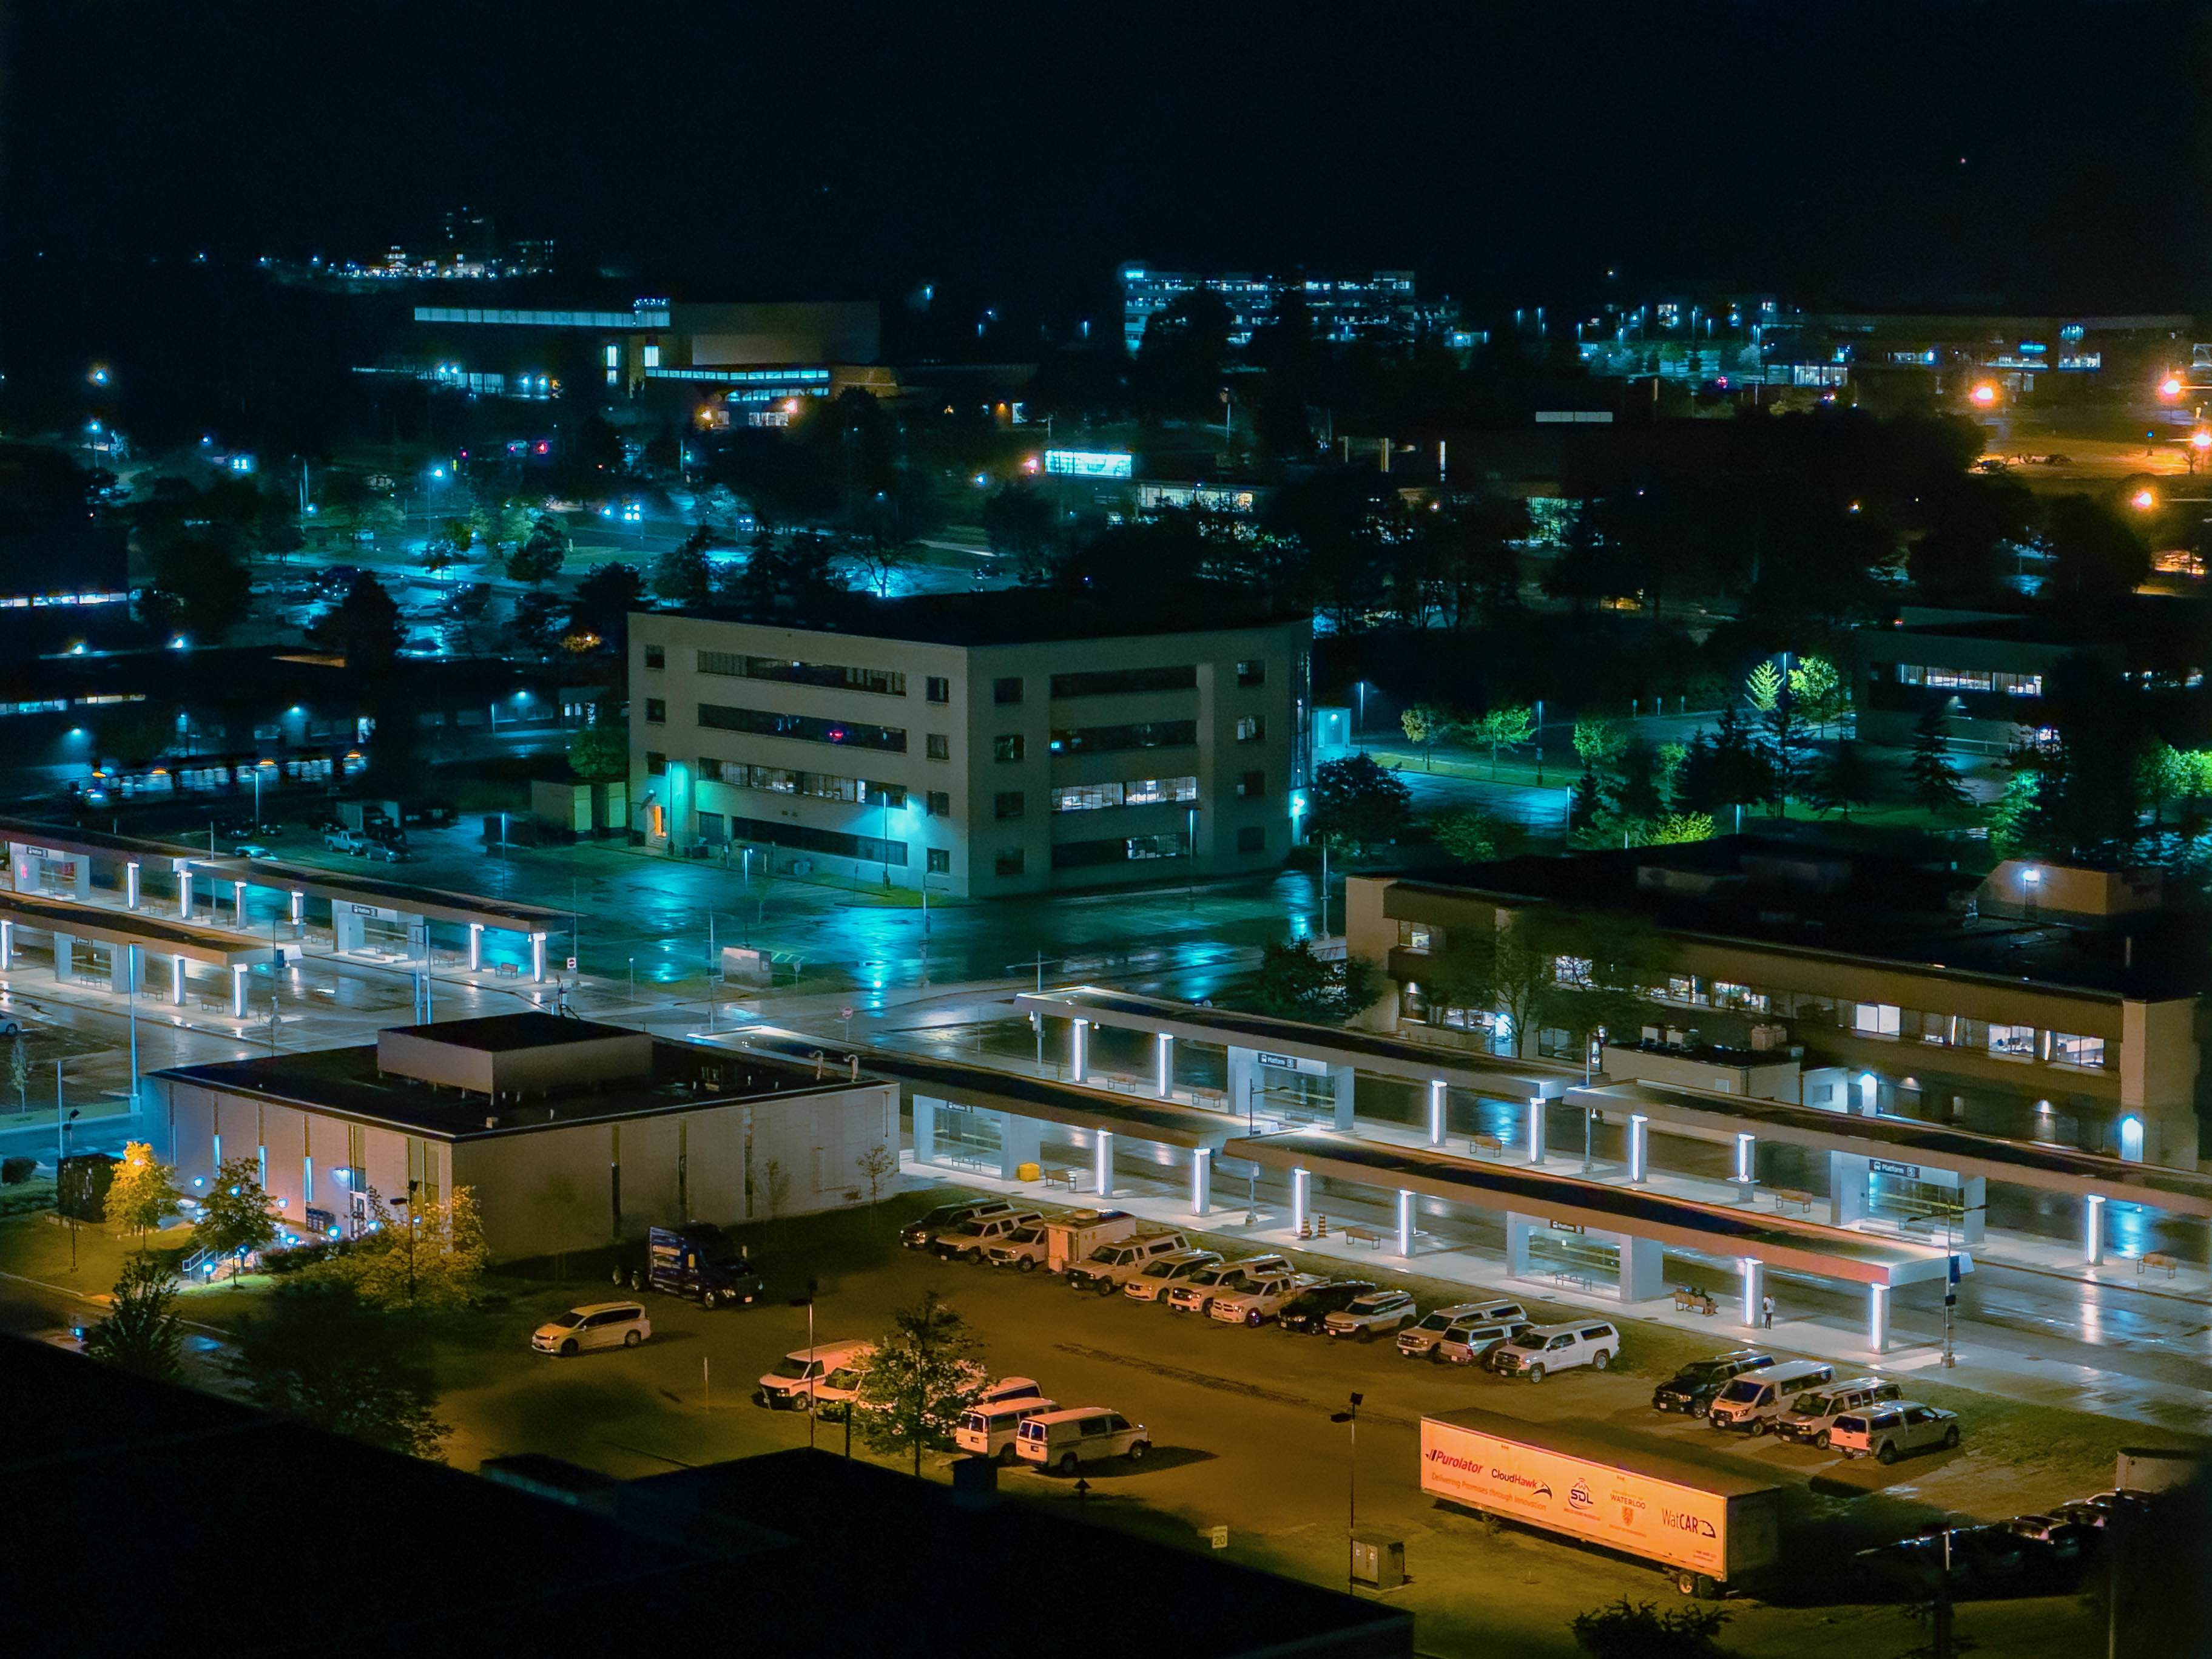
\includegraphics[scale=0.1]{img/loo.jpg}
    \caption{Waterloo, ON}
\end{figure}


\chapter{组合存在性定理}

\section{有限偏序集的分解定理(Dilworth's Theorem)}

{\it to be written}

\section{Pigeonhole Principle}
\ex{
    从1到2n的正整数中,任取n+1个数,至少有一对数,其中一个数是另一个数的倍数。
}

\pf{
    考虑将每个数分解成 $a_i = 2^{b_i}r_i, i = 1,2,...,n+1$. 由于 $1\sim 2n$
    中仅有 $n$ 个奇数,所以存在 $i<j, r_i = j_j$, 则必有 $a_i | a_j$ 或者 $a_j | a_i$.
}

\ex{
    任意 m 个有序的数中存在连续若干个的和是 m 的倍数。
}
\pf{
    考虑前缀和 mod m 的余数即可。
}

\ex{
    $a_1,...,a_{n^2+1}$ 是实数序列,证明:可以选出 $n+1$ 个元素的子序列使得单调增或者单调减。
}


\pf{
    假设选不出长度为 $n+1$ 的单调序列。令 $m_i$ 表示以$a_i$ 为第一个元素的单调{\bf 增}子序列的最长的长度,则 $m_i \le n$. 
    由抽屉原理,存在 $n+1$ 个下标 $i_1,...,i_{n+1}$ 使得 $m_{i_1}=...=m_{i_{n+1}}$.
    如果存在 $1\le s<t\le n+1$, 使得 $a_{i_s} \le a_{i_t}$,则以 $a_{i_s}$ 开头的单调序列可以更长。矛盾。

    因此 $a_{i_1} > a_{i_2} > ... > a_{i_{n+1}}$, 我们得到长度为 $n+1$ 的严格递减序列。
}
\section{Ramsey's Theorem}

一种简单形式,
\prop{红蓝染色$K_9$的边,证明存在红色的$K_4$或蓝色的$K_3$。By convention, $K_n$ is the complete graph of order $n$.}
\begin{proof}
    Claim: 存在一个节点关联至少4条蓝边或者6条红边。

    若否,则图中红边数量不超过 $[\frac{5 \times 9}{2}] = 22$, 蓝边数量不超过 $[\frac{3\times 9}{2}] = 13$, 但是 $K_9$ 有 $C_9^2 = 36$ 条边。矛盾。

    如果 $v_1$ 关联了4条蓝色边,
    \[\begin{tikzcd}
        && {v_1} \\
        \bullet &&&& \bullet \\
        & \bullet && \bullet
        \arrow[color={rgb,255:red,92;green,92;blue,214}, no head, from=1-3, to=2-1]
        \arrow[color={rgb,255:red,92;green,92;blue,214}, no head, from=1-3, to=2-5]
        \arrow[color={rgb,255:red,92;green,92;blue,214}, no head, from=1-3, to=3-2]
        \arrow[color={rgb,255:red,92;green,92;blue,214}, no head, from=1-3, to=3-4]
    \end{tikzcd}\]

    如果上图中4个点之间存在蓝色边,则出现蓝色$K_3$. 若都是红色边,则出现红色$K_4$.

    如果 $v_1$ 关联了6条红色边,考虑这6个点之间的染色,
    \[\begin{tikzcd}
        \bullet && {v_1} && \bullet \\
        \bullet &&&& \bullet \\
        & \bullet && \bullet
        \arrow[color={rgb,255:red,214;green,92;blue,92}, no head, from=1-1, to=1-3]
        \arrow[color={rgb,255:red,214;green,92;blue,92}, no head, from=1-3, to=1-5]
        \arrow[color={rgb,255:red,214;green,92;blue,92}, no head, from=1-3, to=2-1]
        \arrow[color={rgb,255:red,214;green,92;blue,92}, no head, from=1-3, to=2-5]
        \arrow[color={rgb,255:red,214;green,92;blue,92}, no head, from=1-3, to=3-2]
        \arrow[color={rgb,255:red,214;green,92;blue,92}, no head, from=1-3, to=3-4]
    \end{tikzcd}\]
    
    由于2-染色$K_6$必定出现红色或蓝色$K_3$. 如果出现蓝色$K_3$,已经证毕。如果出现红色$K_3$,则和$v_1$组成红色$K_4$.
\end{proof}

\prop{$K_8$不满足上个命题的性质}
\begin{proof}
    \[\begin{tikzcd}
        & \bullet & \bullet \\
        \bullet &&& \bullet \\
        \bullet &&& \bullet \\
        & \bullet & \bullet
        \arrow[color={rgb,255:red,214;green,92;blue,92}, no head, from=1-2, to=1-3]
        \arrow[color={rgb,255:red,214;green,92;blue,92}, no head, from=1-2, to=2-1]
        \arrow[color={rgb,255:red,214;green,92;blue,92}, no head, from=1-2, to=2-4]
        \arrow[color={rgb,255:red,214;green,92;blue,92}, no head, from=1-2, to=3-1]
        \arrow[color={rgb,255:red,214;green,92;blue,92}, no head, from=1-3, to=2-4]
        \arrow[color={rgb,255:red,214;green,92;blue,92}, no head, from=1-3, to=3-4]
        \arrow[color={rgb,255:red,214;green,92;blue,92}, no head, from=2-1, to=1-3]
        \arrow[color={rgb,255:red,214;green,92;blue,92}, no head, from=2-1, to=3-1]
        \arrow[color={rgb,255:red,214;green,92;blue,92}, no head, from=2-1, to=4-2]
        \arrow[color={rgb,255:red,214;green,92;blue,92}, no head, from=2-4, to=3-4]
        \arrow[color={rgb,255:red,214;green,92;blue,92}, no head, from=2-4, to=4-3]
        \arrow[color={rgb,255:red,214;green,92;blue,92}, no head, from=3-1, to=4-2]
        \arrow[color={rgb,255:red,214;green,92;blue,92}, no head, from=3-4, to=4-2]
        \arrow[color={rgb,255:red,214;green,92;blue,92}, no head, from=4-2, to=4-3]
        \arrow[color={rgb,255:red,214;green,92;blue,92}, no head, from=4-3, to=3-1]
        \arrow[color={rgb,255:red,214;green,92;blue,92}, no head, from=4-3, to=3-4]
    \end{tikzcd}\]
    除这些红色边外,其他都连蓝色边。可以验证,图中不存在蓝色三角形$K_3$,不存在红色$K_4$.
\end{proof}

上面两个命题说明9是满足此性质的最小数,$R(3,4) = 9$.

\thmr{Ramsey}{Ramsey}{
    设 $p, q$为正整数,$p, q \ge2$,则存在最小正整数$R(p, q)$,使得当$n \ge R(p, q)$时,用红蓝两色涂色$K_n$ 的
边,则或存在一个蓝色的$K_p$,或存在一个红色的 $K_q$.

}
\begin{proof}
    归纳法。不难看出 $R(p,2) = p, R(2, q) = q$.
    假设 $R(p, q-1), R(p-1,q)$ 存在,我们证明
    \[R(p,q) \le R(p,q-1) + R(p-1, q)\]
    考虑 $n = R(p,q-1) + R(p-1, q)$ 个点的图染色。任取点$v$,则或者$v$于$R(p-1,q)$个点连蓝色边,或者和$R(p,q-1)$个点连红色边(why?)。
    
    如果$v$与$R(p-1,q)$个点连蓝色边。由归纳假设,这$R(p-1,q)$个点中必存在蓝色$K_{p-1}$或红色$K_q$.若为红色$K_q$,已经结束。若为蓝色$K_{p-1}$,则和$v$组成蓝色$K_p$.

    $v$与$R(p,q-1)$个点连红色边的情况同理。
\end{proof}

Ramsey's Theorem 可以用集合的语言表述,进行推广。
\thmr{Ramsey}{RamseyGeneral} {
    对于任意给定的整数 $p,q,r,(p,q \ge r)$, 存在最小的正整数 $R(p,q;r)$, 使得当集合的元素个数 $|S| \ge R(p,q;r)$ 时,将 $S$ 的所有$r$元子集合任意划分成2组($E_1,E_2$), 
    则 

    或者存在 $S$ 的p元子集$A_1$, 使得$A_1$的任意$r$元子集属于$E_1$;

    或者存在 $S$ 的p元子集$A_2$, 使得$A_2$的任意$r$元子集属于$E_2$。
}

下面的例子是广义Ramsey's Theorem的引用。

\ex{
    对任意$\mathbb{N} \ni m \ge 3$, 存在正整数 $N(m)$, 对任意$\mathbb{N} \ni n > N(m)$, 若平面中$n$个点没有三点共线,则存在$m$个点构成一个凸$m$边形的顶点。
}

\begin{proof}
    显然,$N(3) = 3$. 

    {\bf Lemma 1} 验证$N(4) = 5$。考虑5个点的凸包,讨论凸包是三角形还是其他。
    
    Lemma 1说明任意5个以上的点,如果没有三点共线,则存在凸四边形。所以,一个启发是考虑$n$个点中所有4元组,将它们分成两类,一类包含所有凸四边形,一类不包含凸四边形。如果考虑 $R(5,m;r)$ 那么由Lemma 1
    保证存在$m$个点的集合,使得任意四个点都构成凸四边形。
    
    于是很自然的问,

    {\bf Lemma 2} 如果$m$个点中任意4个点构成凸四边形,则这$m$个点构成凸$m$边形。
    
    证明方法:同样考虑凸包和三角剖分即可。

\end{proof}

\chapter{高级计数}

\section{Catalan数}

\defn{Catalan Numbers}{
    第 n 个卡特兰数定义为 $c_n = \frac 1 {n+1}C_{2n}^n$。 

    $c_1 = 1, c_2 = \frac 1 3 C_4^2 = 2, c_3 = \frac 1 4 C_6^3 = 5, c_4 = \frac 1 5 C_8^4 = 14$
}

\prop{

    补充定义 $c_0 = 1$ (如果定义$\binom{0}{0} = 1$), 则Catalan Numbers满足
    \[
        c_n = c_0c_{n-1} + c_1c_{n-2} + ... + c_{n-1}c_0.
    \]
}
\begin{proof}
    考虑生成函数 $f(X) = \sum_{i = 0}^{\infty} c_i X^i$. 


\end{proof}

\ex{
    将一个凸 $n$ 边形三角剖分,方法数记作 $h_{n}$, 证明:$h_{n+2} = c_n$.
}
\begin{proof}
    $h_3 = 1 = c_1$. For $n\ge 4$, take any point $P$, consider which point connects to $P$ or {\bf if $P$ is alone}. This yields
    \[
        h_n = h_3h_{n-1} + h_4 h_{n-2} + ... + h_{n-1}h_3 + h_{n-1}.
    \]

    Another way: consider a segment $P_iP_{i+1}$, which point $P$ connects both $P_i$ and $P_{i+1}$ (i.e., forms a triangle) ? 
    WLOG, we may assume a segment $h_2 = 1$. This yields

    \[
        h_n = h_2h_{n-1} + h_3h_{n-2} + ... + h_{n-1}h_2
    \]

    Consider power series $f(X) = \sum_{i = 0}^{+\infty} h_i X_i$. Assume $h_0 = h_1 = 0$. We have 
    \[
        f(X)^2 = \sum_{n = 3}^{+\infty} l_n X^{n+1}, \text{ where } l_n =  h_2h_{n-1}+...+h_{n-1}h_3 + h_{n-1}h_2 = h_n. 
    \]
    Thus, 
    \[
        f(X)^2 = X (f(X) - X^2)
    \]
    We duduce that 
    \[
        f(X) = \frac 1 2 x\pm \frac 1 2 x (1-4x)^{\frac 1 2} = \frac  1 2 x \pm (\frac 1 2 x - x^2 - x^3 + o(x^3)).
    \]
    Therefore, $f(X) = \frac 1 2 x - \frac 1 2 x(1-4x)^{1/2}$. And 
    \[
        h_{n+1} = \frac 1 2 \left| \binom{\frac 1 2}{n} 4^n\right| = \frac {\binom{2(n-1)}{n-1}} n = c_{n-1}.
    \]
\end{proof}

\ex{
    {\bf 括号序列的一般版本} 给定$n\ge m$, 求$n$个a和$m$个b的排列个数,使得任意 $1\le k \le n+m$, 前$k$个字符中 $a$ 的个数不少于 $b$ 。
}
\begin{proof}
    设无限制条件时的排列集合为 $U$, 则 $|U| = \binom{n+m}{n}$. 

    设不满足条件时的组合数的排列集合为 $V$, 即存在某个 $k$, 使得前 $k-1$ 个数,恰好有一半的$a$和$b$,但第$k$个数$b$. 将前 $k$ 个数中a,b反转,则得到了$n+1$个$a$, $m-1$个$b$的排列。

    设$(n+1, m-1)$的无限制条件的排列集合为$W$. 

    {\bf claim: 上述变换是 $V \to W$ 的bijection.} 
    因此 $|V| = \binom{n+m}{n+1}$.
\end{proof}

\begin{remark}
    在上述例子中, 取 $m = n$, 得到排列数为 $c_n = \frac {\binom{2n}{n}} {n+1} = \binom{2n}{n} - \binom{2n}{n+1}$
\end{remark}
\begin{remark}
    上述例子也相当于平面直角坐标系中,从(0,0)出发,每一步向右走,纵坐标可以+1或-1,即 $(x,y) \to (x+1, y\pm 1)$, 但不允许出现 $x>0,y = 0$(即必须始终在y轴上方)的限制下, 从(0,0)到(n+m,n-m)的路径数。
\end{remark}

\ex{
    2n个点分布在圆周上,用n条不相交的弦配对的方法数为$c_n$.
}
\ex{
    $1,2,...,n$按先后顺序进入stack后出stack的可能顺序为$c_n$.
}

\begin{proof}
    仿照3.1.2,用生成函数即可。
\end{proof}

\section{第一类Stirling数}

下面给出三种定义,证明它们是等同的。

\defn{定义1}{
    $f(X) = X(X-1)(X-2)...(X-n+1)$ 的展开式中 $X^r$ 的系数的绝对值定义为 $n \brack r$
}
\defn{定义2}{
    $f(X) = X(X+1)(X+2)...(X+n-1)$ 的展开式中 $X^r$ 的系数定义为 $n \brack r$
}

\defn{定义3: 组合意义,Stirling轮换数}{
    表示将 n 个两两不同的元素,划分为 r 个互不区分的非空轮换的方案数,定义为 $n\brack r$

    等价描述:$S_n$中可以拆成$r$个不交轮换的置换个数为$n\brack r$.
}

\begin{proof}
    定义1,2等同容易验证。
    
    定义3给出了递推公式:考虑前 $n-1$ 个元素划分成多少个非空轮换,
    \begin{itemize}
        \item 若为$r-1$个,则第n个元素单独构成一个轮换。共有$n-1\brack {r-1}$ 个。
        \item 若为$r$个,考虑将第n个元素插入其中一个轮换。共有${n-1\brack r} \cdot (n-1)$个。
    \end{itemize}
    因此 \[{n\brack r} = {n-1\brack r-1} + {n-1\brack r}\cdot (n-1)\]

    我们证明定义2也可以导出这个递推式:
    考虑 $X^r$ 的系数有没有取 $(X+n-1)$中的$n-1$。如果取了,贡献为 $(n-1)\cdot {n-1\brack r}$; 如果没取,贡献为 $n-1\brack r-1$. 从而递推式是相同的。

    定义3中,可以符合直观的规定$r>n$时, ${n\brack r} = 0$, ${n\brack 0} = 0$. 那么可以验证,$\forall n,r \ge 0$, 递推公式都成立。 
    
    定义3也可从组合意义得出${n\brack n}= 1, {n\brack 1} = (n-1)!$的边界条件。
    
    定义2中同样可以导出相同的边界条件。

    因此3个定义是等同的。
\end{proof}

\begin{figure}[H]
    \center
    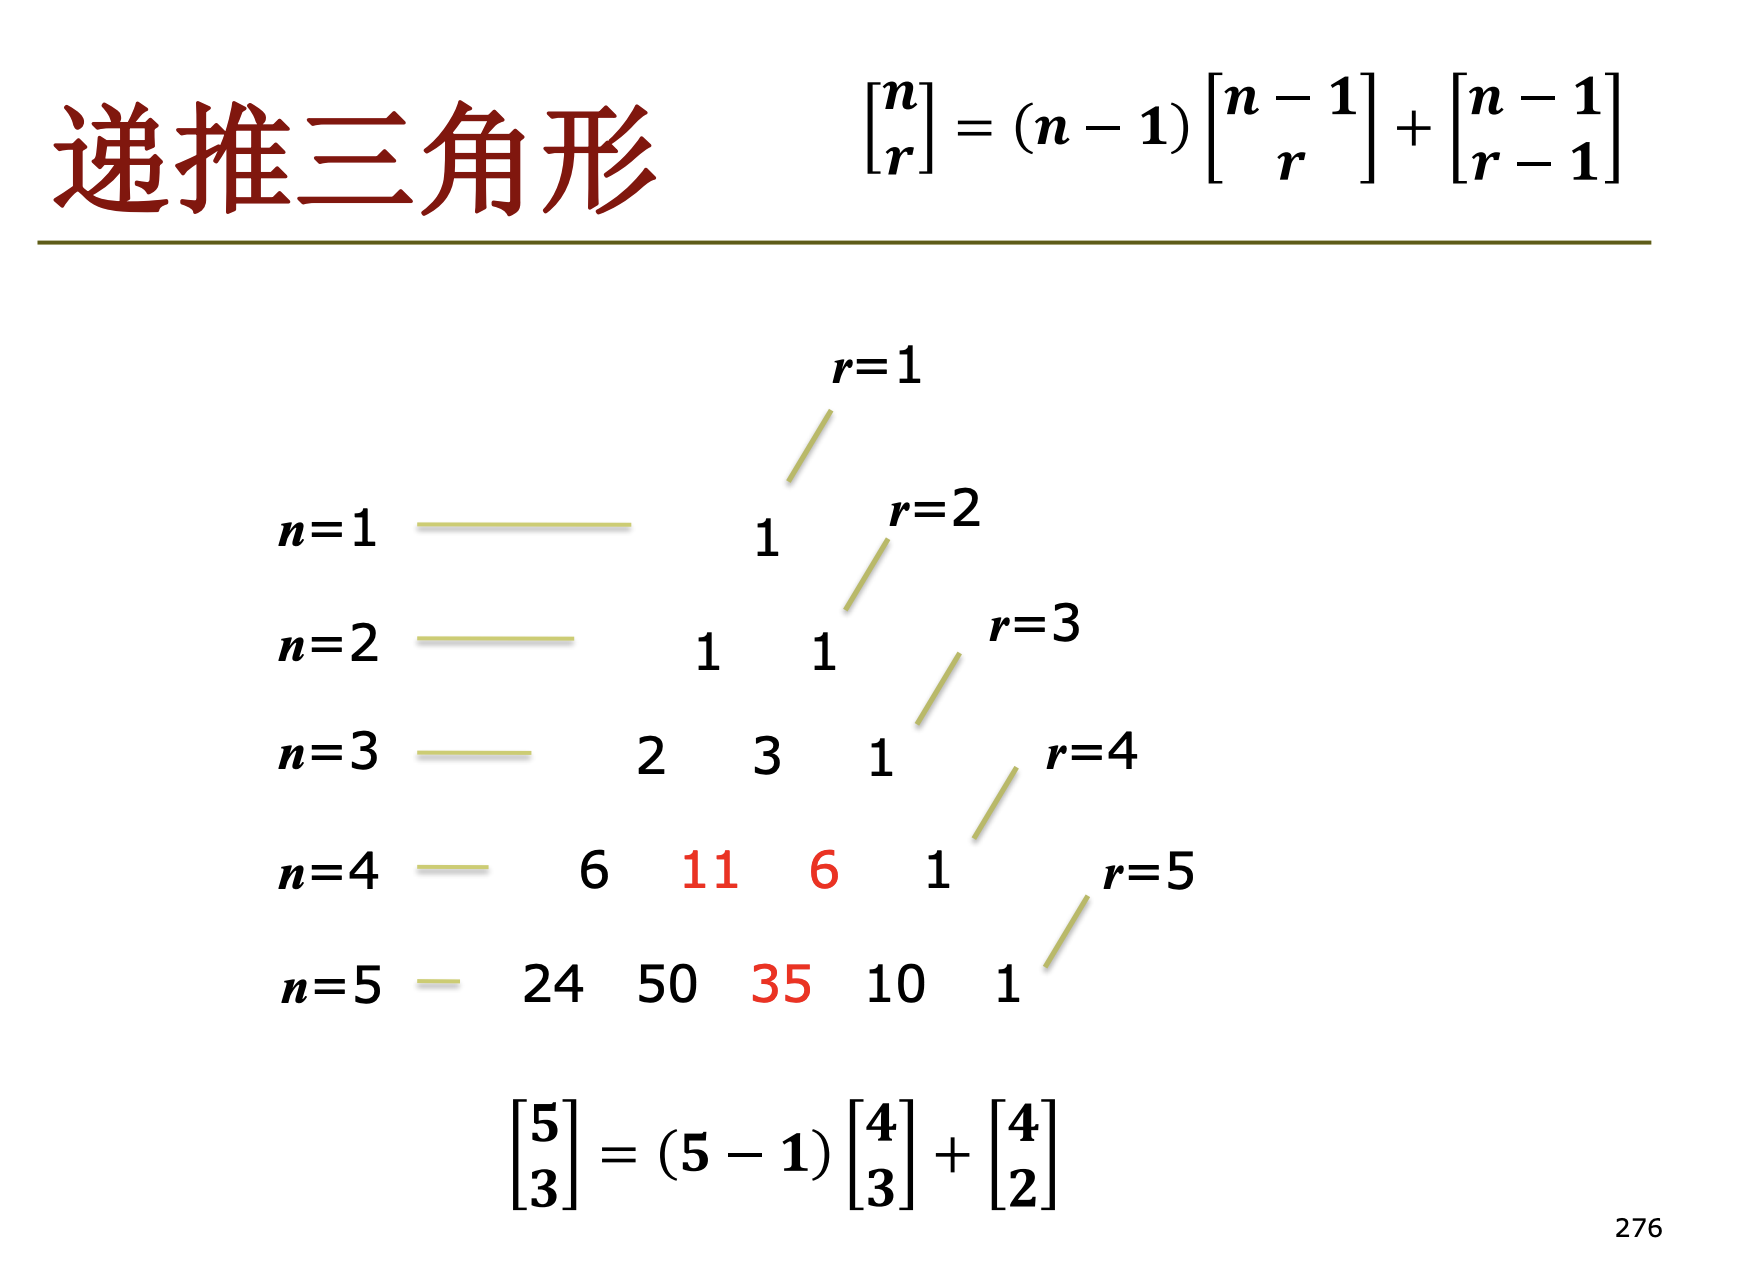
\includegraphics[scale=0.5]{img/stirling1.png}
\end{figure}

\prop{
    在定义2中代入 $X = 1$ 得到 
    \[
        \sum_{i = 1}^{n} {n\brack i} = n!
    \]

    考虑 $X_{n-1}$ 的系数,得到
    \[
        {n\brack n-1} = 1 + 2 + ... + (n-1) = \binom{n}{2}
    \]
}

\section{第二类Stirling数}

\defn{}{
    $n$个两两不同的元素划分的$r$个非空子集的方法数。记为 $n\brace r$

    等价描述:n个不同的球恰好放到r个相同的盒子里的方法数。

    约定边界条件:
    \begin{itemize}
        \item $r > n$ 时, $n\brace r$ = 0.
        \item $n\brace n$ = 1, $n\brace 0$ = 0.
    \end{itemize}
}

\prop{
    \[
    {n\brace r} = {n-1\brace r-1} + r{n-1\brace r}
    \]
}
\begin{proof}
    考虑组合意义。先划分前n-1个元素。
\end{proof}

\prop{
    (1) ${n\brace 1} = 1$


    (2) $n \brace 2$ = $2^{n-1}-1$.

    用递推式不断展开会发现:$n \brace 2$ = $2^{n-2} {2\brace 2} + 2^{n-3} {2\brace 1} + 2^{n-4}{3\brace 1} + ... + 1\cdot {n-1\brace 1}$

    (3)

    \[
    \sum_{n_1 + ... + n_m = n,\forall n_i > 0} \binom{n}{n_1 \ n_2 \ ... \ n_m} = m!{n\brace m}
    \]

    组合意义:n个不同的球分到m个不同的箱子,{\bf 且每个箱子非空}的方法数。

    Note: 如果允许空箱子,这个过程也可以看作n个元素中,每一个任意选箱子放进去。从而得到
    \[
    \sum_{n_1 + ... + n_m = n,\forall n_i \ge 0} \binom{n}{n_1 \ n_2 \ ... \ n_m} = m^n
    \]

    (4)
    \[\sum_{k=1}^{m}\binom{m}{k}{n\brace k} k! = m^n \]

    组合意义,先选k个非空箱子来放,再区分这k个箱子。

    (5)

    \[
    {n+1\brace r} =\sum_{k=0}^{n}\binom{n}{k} {k\brace r-1}
    \]

    组合意义:讨论第n+1个球和哪些球放在一个箱子中。

    (6) n个球放入m个不区分的盒子,允许空盒的方法数为
    \[\sum_{k=1}^{m}{n\brace k}\]
}

\prop{
    第二类Stirling数有通项公式:
    \[
    {n\brace m} = (-1)^m \sum_{i=1}^{m} \frac {(-1)^i \cdot i^n}{i!(m-i)!}
    \]
    这个式子可以通过卷积计算。
}

\begin{proof}
    比如 ${4\brace 2} = 7$可以验证:$(-1)^2 (-\frac 1 1 + \frac {16} 2) = 7$ 

    证明将用到二项式反演, 
\end{proof}

\lem{Binomial Inversion Formula}{
    Let's say that we have the equation for any $k\ge 0$:
    \begin{equation}
        f_k = \sum_{i=0}^{k}\binom{k}{i} g_i
    \end{equation}
    
    Prove that $g_k$ can be expressed in the combination of $\{f_i\}$ as the following form:
    \begin{equation}
        g_k = \sum_{i = 0}^{k}(-1)^{k-i}\binom{k}{i}f_i 
    \end{equation}
}

\begin{proof}
    For $0\le i\le k$, calculate how many $f_i$ (denoted as $l_i$) in the RHS of (3.1), if we admit (3.2).

    \[
        l_i = \sum_{j=0}^{k}\binom{k}{j}(-1)^{j-i}\binom{j}{i}
    \]    
    When $i = k$, we easily get $l_k = 1$.

    When $i < k$, we induce on $k$. Suppose $k-1$ holds, then 

    \[
    (-1)^j \binom{k}{j}\binom{j}{i} = (-1)^j\binom{k-1}{j}\binom{j}{i} + (-1)^j\binom{k-1}{j-1}\binom{j-1}{i} + (-1)^j\binom{k-1}{j-1}\binom{j-1}{i-1}
    \]
    Sum over all $j =0,...,k$, we have
    \[
    l_i = \underbrace{\sum_{j=0}^{k}(-1)^j\binom{k-1}{j-1}\binom{j-1}{i-1}}_{=0} + \underbrace{\sum_{j=0}^{k}(-1)^j \binom{k-1}{j}\binom{j}{i} + \sum_{j=0}^{k}(-1)^j \binom{k-1}{j-1}\binom{j-1}{i}}_{\text{正负相反,=0}}
    \\ = 0
    \]
\end{proof}

\begin{proof}
    {\bf Proof of Propsition 3.3.4}

    n 个两两不同的元素,划分到 i 个两两不同的集合(允许空集)的方案数为 $G_i$.

    n 个两两不同的元素,划分到 i 个两两不同的非空集合的方案数为 $F_i$.

    则 $G_i = i^n$, 且由Propositon 3.3.3, 
    \begin{equation}
        F_i = i!\cdot{n\brace i} 
    \end{equation}

    \begin{equation}
        G_i = \sum_{j = 0}^{i}\binom{i}{j}F_j.
    \end{equation}
    
    因此由二项式反演:

    \begin{align}
            \frac {F_m}{m!} &= \frac 1 {m!}\sum_{j=0}^{m}(-1)^{m-j}\binom{m}{j}G_j \\
                &= \frac 1{m!}\sum_{j=0}^{m}(-1)^{m-j}\binom{m}{j}j^n\\
                &= (-1)^m\sum_{j=0}^{m}\frac {(-1)^jj^n} {j!(m-j)!}
    \end{align}

\end{proof}

\chapter{组合计数定理}

\section{容斥原理}

\thm{容斥原理}{
设$S$为非空有穷集,$A_i \subset S, \forall i \le n$, 则
\[
    \left|\overline{A_1}\cap\overline{A_2}\cap...\cap\overline{A_n}\right| = |S|+\sum_{k=1}^{n} (-1)^k\sum_{i_1<i_2<...<i_k} \left|A_{i_1}\cap A_{i_2}\cap...\cap A_{i_k}\right|
\]
}

\cor{
    设$S$为非空有穷集,$A_i \subset S, \forall i \le n$, 则
    \[
    \left|A_1\cup A_2\cup...\cup A_n\right| = \sum_{k=1}^{n} (-1)^{k-1}\sum_{i_1<i_2<...<i_k} \left|A_{i_1}\cap A_{i_2}\cap...\cap A_{i_k}\right|
\]
}

\begin{proof}
    统计属于 $k$ 个集合的元素对等式两边的贡献即可。
\end{proof}

\ex{
    {\bf 多重集的r组合数}

    $B = \{3\cdot a, 4\cdot b, 5\cdot c\}$ 的10-组合数。
}

\ex{
    {\bf 交错和的恒等式}

    For $r \ge m$, prove that 
    \[
        \binom{n-m}{r-m} = \sum_{i=1}^{m}(-1)^i\binom{m}{i}\binom{n-i}{r}
    \]
}
\begin{proof}
    Let $S = \{1,2...,n\}, A = \{1,2...,m\}$. 计数包含$A$的$S$的$r-$组合数。令 $P_j$ 表示不包含 $j$ 的r-组合数的集合。
\end{proof}

\ex{
    {\bf 错位排列}

    用 $D_n$ 表示 n 个元素的错位排列的方案数。求$D_n$.
}
\begin{proof}
    $D_n = n! - \binom{n}{1}(n-1)! + \binom{n}{2}(n-2)! + ... = n!(1 - \frac 1{1!} + \frac 1{2!} + ... + (-1)^{n}\frac 1 {n!})$
\end{proof}

\section{棋盘多项式}

给定一张棋盘 $C$, 放 $k$ 个棋子。每行每列至多一个棋子。求方案数。

定义:

\begin{figure}[H]
    \center
    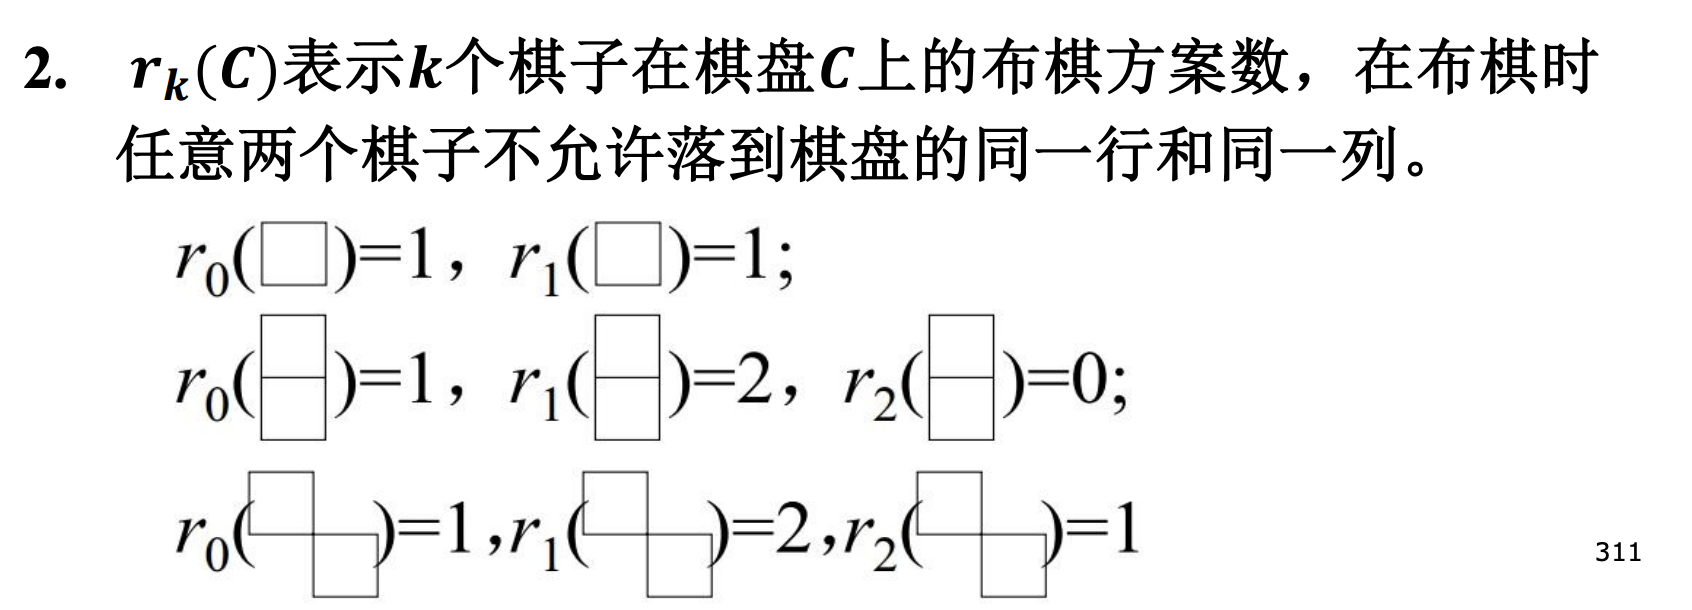
\includegraphics[scale=0.4]{img/chess1.png}
\end{figure}

我们约定 for any $C$, $r_0(C) = 1$

\prop{
    (1) $r_1(C) =$ C的方格数。 

    (2)
    设$C_i$是从棋盘中去掉指定的方格所在的行和列后剩余的棋盘,
    $C_l$是从棋盘中去掉指定的方格后剩余的棋盘,则

    \[
        r_k(C) = r_{k-1}(C_i) + r_k(C_l)
    \]

    (3)设棋盘$C$由两个子棋盘$C_1$和$C_2$构成,如果$C_1$和$C_2$没有公共的行
和列,则

\[
    r_k(C) = \sum_{i = 0}^{k} r_i(C_1)r_{k-i}(C_2)
\]
}

\defn{棋盘多项式}{
    定义 $R(C) = \sum_{i=0}^{\infty}r_i(C)X^i$
}

\prop{
    (1)对于任意一个格子,可以得到 $C_i, C_l$, 则
    \[
        R(C) = xR(C_i) + R(C_l)
    \]

    (2)设棋盘$C$由两个子棋盘$C_1$和$C_2$构成,如果$C_1$和$C_2$没有公共的行
    和列,则
    \[
        R(C) = R(C_1)\cdot R(C_2)
    \]
}

\begin{figure}[H]
    \center
    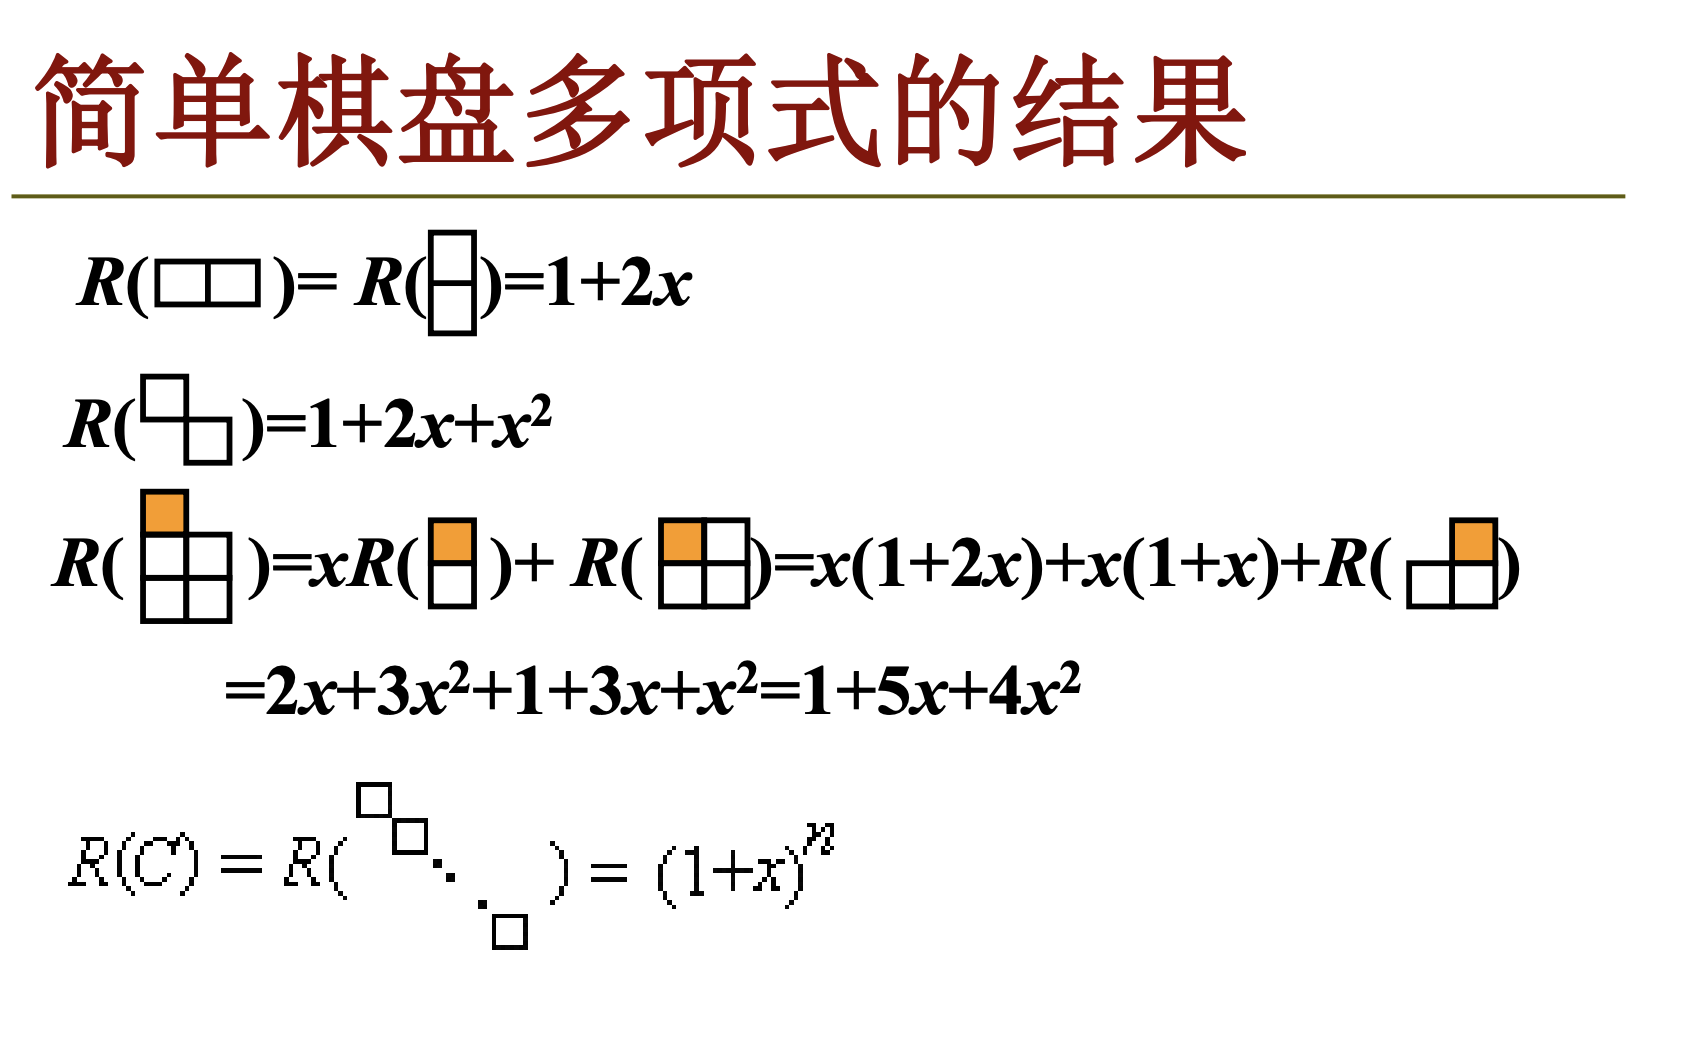
\includegraphics[scale=0.5]{img/chess2.png}
\end{figure}

\subsection{棋盘多项式的应用--有禁区的排列}

\thm{}{
    $C$ 是给定 $n\times n$ 棋盘的禁区。设棋盘多项式为 $R(C) = \sum_{i = 0}^{\infty}r_iX^i$. 则有禁区的排列数为 
    \[
        l = \sum_{i=0}^{n}(-1)^i r_i(n-i)! = n! - r_1(n-1)! + r_2(n-2)! + ... +(-1)^nr_n 
    \]
}

\ex{用上述定理证明错排公式}
\begin{proof}
    设 $C$ 为只有对角元的棋盘,则 $R(C) = (1+x)^n = \sum_{i=0}^{n}\binom{n}{i}x^i$.
    代入定理得,

    \[
        D_n = \sum_{i=0}^{n}(-1)^i \binom{n}{i}(n-i)! = n!\left(\sum_{i=0}^{n}(-1)^i\frac 1 {i!}\right)
    \]
    
\end{proof}


% \end{CJK}
\end{document}
